%%% Template para anotações de aula
%%% Feito por Daniel Campos com base no template de Willian Chamma que fez com base no template de  Mikhail Klassen
%%% Versão atual editada por Giovanna de Lima

\documentclass[12pt,a4paper, brazilian]{article}

%%%%%%% INFORMAÇÕES DO CABEÇALHO
\newcommand{\workingDate}{\textsc{\selectlanguage{portuguese}\today}}
\newcommand{\userName}{ET645}
\newcommand{\institution}{UFPE}
\usepackage{researchdiary_png}
\usepackage{wrapfig}
\usepackage{booktabs}
\usepackage{caption}
\usepackage{titlesec}

\titleformat{\section}
{\normalfont\fontsize{15}{19}\bfseries}
{\thesection}{1em}{}

\titleformat{\subsection}
{\normalfont\fontsize{13}{19}\bfseries}
{\thesubsection}{1em}{}

\captionsetup{font=small, labelfont=bf, labelsep=period}

\begin{document}

\begin{center}
{\fontsize{12}{10}\selectfont\textbf{REDES NEURAIS}}\\[4mm]
{\fontsize{18}{20}\selectfont\textbf{Aplicação de Redes Neurais Convolucionais (CNNs)}}\\[2mm]
{\fontsize{18}{20}\selectfont\textbf{na classificação de manobras de Surf}}\\[3mm]
{\fontsize{14}{15}\selectfont Giovanna de Lima}\\[3mm]
\today\\[5mm] %% se quiser colocar data
\end{center}

\section{Introdução}

No treinamento de praticantes do surf, sobretudo atletas de alta-performance, a análise de vídeo é uma ferramenta essencial para identificação de falhas técnicas e de execução, proporcionando meios para evolução guiada do surfista. Um grande volume de material de gravação é produzido numa sessão de surf, podendo incluir diferentes manobras com execução completa ou incompleta, além de falhas no momento de entrada na onda (não gerando manobras para análise posterior). Muitas vezes, as gravações produzidas devem ser filtradas manualmente, removendo vídeos de baixa-qualidade, separando manobras por pasta e, por fim, avaliando a qualidade da execução com base na \textit{expertise} do treinador. Esse processo não é apenas demorado, mas também difícil para surfistas que não possuem um treinador pessoal para realizar tal avaliação, frequentemente impossibilitando a extração de informações relevantes das gravações.
    
Com o avanço de técnicas de inteligência artificial, sua utilização no campo dos esportes é crescente, sobretudo em aplicações de visão computacional \cite{Eric2024-ie, Fu2025-vz}. Nesse contexto, destacam-se as Redes Neurais Convolucionais (CNNs), um modelo computacional bioinspirado capaz de aprender padrões visuais em dados estruturados como imagens \cite{Baccouche2011-kw}. Elas são capazes de realizar tarefas como detecção de objetos, classificação de vídeos e rotulagem de cenas {\cite{KarpathyCVPR14}}, de forma automática e em larga-escala, desde que o treinamento da rede seja realizado num banco de dados adequado à tarefa que deseja ser executada. Um exemplo da aplicação de redes neurais no contexto do surf é fornecido pela empresa Flowstate, que treinou uma CNN em milhares de gravação de manobras em piscinas de onda, permitindo a detecção e separação automática das manobras de um surfista que utiliza seus serviços \cite{shaw2026flowstate}. Outras aplicações em desenvolvimento incluem a extração de variáveis objetivas para avaliação da qualidade da manobra, como: compressão do corpo, velocidade, força, torque, entre outros \cite{flysurfAISurfing}. Nesse caso, embora uma CNN não seja a arquitetura ideal para extração de características interpretáveis, sua aplicação está relacionada à classificação da manobra executada, permitindo que as variáveis obtidas sejam comparadas com parâmetros específicos ao movimento identificado. 
        
Sendo assim, o presente trabalho busca aplicar uma arquitetura de Rede Neural Convolucional para classificação de manobras de surf. Para isso, será utilizando o banco de dados "\textit{Surf Maneuvers Recognition}", que inclui 1062 gravações de manobras distribuídas em quatro classes: \textit{360}, \textit{cutback-frontside}, \textit{roller} e \textit{take-off}. Além disso, será avaliada a performance do modelo criado com base em métricas objetivas, buscando compreender as possibilidades e limitações de CNNs aplicadas à classificação de vídeos.

\section{Fundamentos Teóricos e Metodológicos}

\subsection{Redes Neurais Convolucionais}

\begin{wrapfigure}{l}{0.27\textwidth}
    \centering
    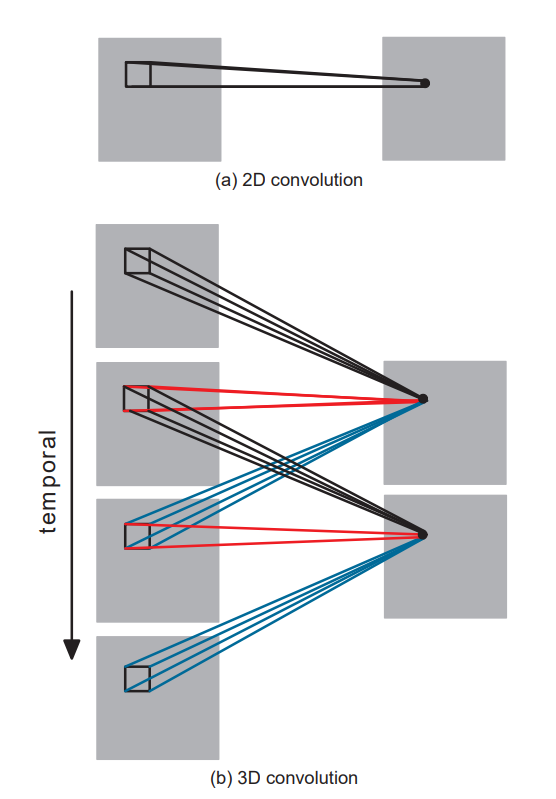
\includegraphics[width=\linewidth]{figuras/conv3d.png}
    \caption{Convolução \\3D esquematizada. \\ Fonte: \cite{Ji2013-lv}}
    \label{fig:conv3d}
\end{wrapfigure}

Redes neurais são modelos computacionais bioinspirados capazes de aprender características de um conjunto de dados por meio de conexões entre múltiplas camadas de neurônios. Redes Neurais Convolucionais, em particular, extraem características diretamente dos pixels de uma imagem, minimizando drasticamente a necessidade de pré-processamento dos dados e preservando a relação espacial entre pixels. Sua arquitetura é composta por camadas sucessivas de convoluções (executam a extração de características a partir da aplicação de \textit{kernels}) e \textit{pooling} (uma estratégia de subamostragem por meio da redução de dimensionalidade dos dados), contendo pesos treináveis a cada execução da rede {\cite{Baccouche2011-kw}}. Tais camadas, quando associadas a camadas densas de neurônios e funções de ativação que introduzem não-linearidade dos dados, permitem a aplicação da CNN no problema-alvo, como a identificação de um objeto numa imagem. Quando aplicadas no processamento de vídeos, a dimensão temporal dos dados deve ser considerada, e a rede passa a ser chamada de CNN tridimensional (ou CNN 3D). Nesse caso, as camadas de convolução e \textit{pooling} passam a ser executadas com janelas cúbicas, como mostrado na Fig. {\ref{fig:conv3d} {\cite{Ji2013-lv}. Essa adaptação permite que a rede capture padrões que se propagam entre os diferentes frames de um vídeo, como informação de movimento. 

\subsection{Pré-processamento do banco de dados}

\begin{wrapfigure}{r}{0.5\textwidth}
    \centering
    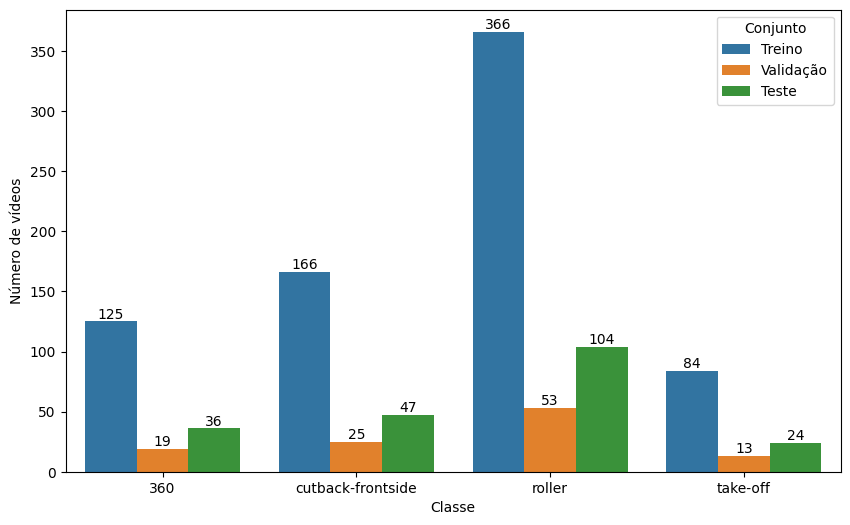
\includegraphics[width=\linewidth]{figuras/class_distribution.png}
    \caption{Distribuição das amostras por classe.}
    \label{fig:class_distribution}
\end{wrapfigure}

 As etapas de carregamento e processamento de dados citadas a seguir foram baseadas majoritariamente no tutorial ``Load video data''  disponibilizado pelo TensorFlow \cite{tensorflowLoadVideo}. O banco de dados ``Surf Maneuvers Recognition'' \cite{twonziiSurfManeuvers}, obtido no Kaggle, contém uma divisão prévia em conjuntos de treino, validação e teste, entretanto, suas classes são desbalanceadas (Fig. \ref{fig:class_distribution}) e os vídeos contém durações distintas. Como a entrada da rede deve ser equivalente entre as observações, foram selecionados e extraídos aleatoriamente 16 frames de cada vídeo, com um passo de 2 frames entre eles. Os valores foram definidos com base na menor duração das gravações, de modo a evitar \textit{black-padded} frames anexados ao final do conjunto. Os frames extraídos foram redimensionados para (128, 128), com preenchimento de barras pretas para preservar a proporção, e associados à classificação da pasta que os originou, com as classes organizadas em ordem alfabética. Em cada frame, foi aplicada a conversão de BGR para RGB e a normalização dos pixels no intervalo entre 0 e 1.

\textit{Data augmentation} é uma estratégia que consiste em aplicar transformações em dados pré-existentes, complementando o \textit{ \textit{dataset} } trabalhado e garantindo maior diversidade dos dados \cite{murel2024dataaugmentation}. Neste trabalho, essa etapa foi realizada com base na metodologia descrita por \textcite{KarpathyCVPR14}, visando reduzir o \textit{overfitting}. Nos dados de treino, foi selecionado aleatoriamente um recorte de (112, 112) a partir do frame redimensionado (128, 128). Esse processo, aplicado uniformemente a todos os frames de um mesmo vídeo em cada época, foi seguido de uma inversão horizontal da imagem com p = 50\%, garantindo que o modelo seja capaz de reconhecer a manobra nas duas direções da onda. Por fim, a média dos valores dos pixels (calculada como 0,294) foi subtraída de todos os frames. Já nos dados de validação e teste, foram aplicados somente um recorte central de (112, 112) e a mesma subtração da média, sem componentes aleatórios, garantindo reprodutibilidade das avaliações.

Em seguida, cada conjunto foi dividido em \textit{batches} de oito clipes (no conjunto de treino, com composição aleatória a cada época). Para reduzir de forma considerável o tempo de execução, os clipes carregados na primeira época foram armazenados em \textit{cache}. Essa estratégia tem a desvantagem de fixar, para cada vídeo, o mesmo conjunto de 16 frames em todas as épocas, possivelmente excluindo trechos mais relevantes para a identificação da manobra. As transformações do \textit{data augmentation}, porém, são aplicadas após o \textit{cache}, de modo que o recorte e a inversão continuam variando a cada época. A execução com e sem \textit{cache} foi comparada, e o pequeno ganho de acurácia obtido não justificou um aumento de cerca de duas horas no tempo de execução.

\subsection{Descrição do modelo}

O modelo avaliado foi adaptado a partir dos tutoriais de Redes Neurais Convolucionais 3D das plataformas TensorFlow \cite{tensorflowVideoClassification} e GeeksForGeeks \cite{geeksforgeeksVideoClassification}. As camadas, construídas com a biblioteca Keras \cite{chollet2015keras}, foram organizadas em três blocos, cada um composto por: Conv3D (kernel de tamanho (3, 3, 3), \textit{padding same}), MaxPooling3D (tamanho (2, 2, 2), \textit{padding same}),  \textit{BatchNormalization} e ativação ReLU. O número de filtros das camadas convolucionais foi aumentado progressivamente entre os blocos (64, 128 e 256, respectivamente). Em seguida, a saída do último bloco foi achatada (\textit{Flatten}) e fornecida a uma camada \textit{Dense} com 512 neurônios e ativação ReLU, seguida de dropout com taxa de 0,5. Por fim, a camada de saída era composta por 4 neurônios com ativação \textit{softmax}, adequada para classificação multiclasse.

Na execução do modelo, foi utilizado o otimizador Adam ($\eta$ = 0,0001), função de perda \textit{Categorical Crossentropy} e pesos personalizados para cada classe, visando combater o problema do desbalanceamento. Os pesos foram calculados com base na eq. \ref{eq:pesos} e normalizados pela média.

\begin{equation}
\label{eq:pesos}
Peso = \frac{1}{\sqrt{n}}
\qquad
\text n \text{ = o número de entradas da classe no conjunto de treino}
\end{equation}
\vspace{0.3em}

O aprendizado do modelo foi acompanhado a partir das métricas de acurácia e F1-score. O treinamento percorreu 100 épocas e os parâmetros da melhor época foram salvos com base no valor máximo de F1-score, sendo utilizados na validação do modelo no conjunto de teste. Ao final, as avaliações do modelo incluíram o acompanhamento das métricas de F1-score e acurácia ao longo das épocas, com posterior validação no conjunto de teste. Ainda, foram calculados a matriz de confusão e as métricas por classe (recall, precisão e F1-score).

\section{Aplicação}

A Fig. {\ref{fig:f1score_epoca}} revela a evolução do F1-score ao longo das 100 épocas de treinamento da rede. O comportamento similar entre os conjuntos de treino e validação revela que as estratégias de redução do \textit{overfitting} foram bem-sucedidas. Mesmo com múltiplas execuções da rede, não foi possível alcançar valores de F1-score superiores a 0,80, revelando um limite superior que possivelmente só pode ser ultrapassado com mudanças no modelo ou no processamento dos dados. Ainda, é relevante citar que o valor de 1062 entradas do  \textit{dataset}  utilizado é pequeno com relação aos modelos de CNN 3D mais precisos, que utilizam dezenas ou centenas de milhares de dados no treinamento da rede, e portanto pode não ser possível elevar drasticamente a acurácia sem a ampliação e o tratamento do banco de dados. 

\begin{wrapfigure}{l}{0.45\textwidth}
    \centering
    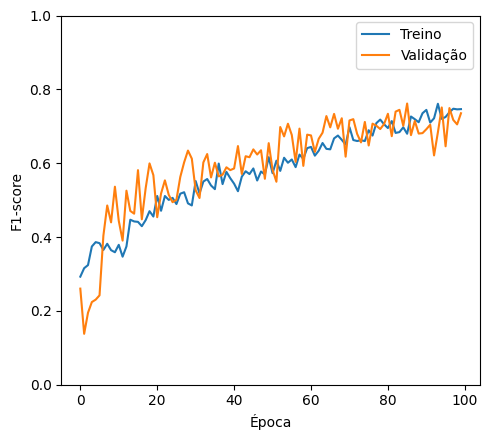
\includegraphics[width=\linewidth]{figuras/plot_epocas_f1.png}
    \caption{Evolução do F1-score médio ao longo das épocas para o conjunto de treino (azul) e validação (laranja).}
    \label{fig:f1score_epoca}
\end{wrapfigure}

Para uma investigação mais detalhada do comportamento classificativo da rede, é disponibilizada a matriz de confusão obtida no conjunto de teste (Fig. ~\ref{fig:matriz_conf}). A matriz evidencia a distribuição desbalanceada das classes e como ela pode ter influenciado os erros de classificação (mesmo com aplicação de pesos distintos no treinamento), visto que os dois blocos de erros com maior número de entradas referem-se à confusão das classes 360 e \textit{cutback-frontside} com a classe mais abundante, \textit{roller}. Em termos de execução, as manobras \textit{roller} e \textit{cutback-frontside} são as mais similares do grupo, visto que ambas são realizadas com mudança de direção entre o \textit{pocket} e o \textit{lip} (crista) da onda, enquanto o 360 é uma manobra majoritariamente aérea e o \textit{take-off} representa apenas a rápida transição entre a remada e a entrada do surfista na onda. Entretanto, a maior confusão ocorreu entre as manobras de 360 e \textit{roller}, o que indica que o modelo pode estar capturando mais fortemente o movimento de subida do surfista na onda do que a execução momentânea da manobra, já que as duas são precedidas por uma trajetória semelhante em direção ao \textit{lip}.

\begin{wrapfigure}{r}{0.53\textwidth}
    \centering
    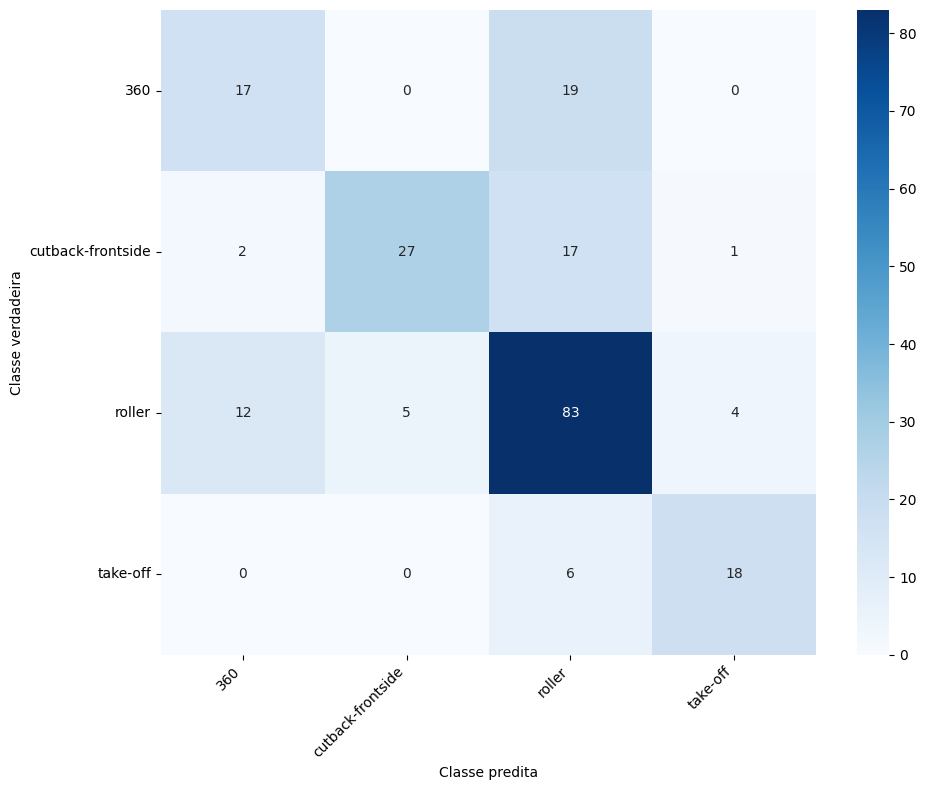
\includegraphics[width=\linewidth]{figuras/matriz_conf.png}
    \caption{Matriz de confusão dos dados de teste.}
    \label{fig:matriz_conf}
\end{wrapfigure}

O relatório de classificação exposto na Tabela~\ref{tab:classification_report} permite compreender mais profundamente o desempenho do modelo em cada classe. A maior precisão ocorre para a classe \textit{cutback-frontside}, o que indica que o modelo está correto em 84\% das vezes que prevê esta manobra. Já no caso do \textit{recall}, que quantifica a porcentagem de exemplos identificados corretamente em cada classe, as manobras \textit{roller} e \textit{take-off} são as mais bem classificadas. Com o maior valor de F1-score, a manobra \textit{take-off} possui o melhor equilíbrio entre \textit{precision} e \textit{recall} no modelo. Já a manobra 360 é a pior classificada em todas as métricas, revelando uma dificuldade do modelo em identificá-la corretamente. É possível que isso esteja relacionado com a baixa quantidade de amostras, embora outras justificativas também devam ser consideradas, já que a classe menos abundante (\textit{take-off}) é muito melhor representada. O alto \textit{recall} (0,80) em contraste com a precisão moderada (0,66) da classe \textit{roller} indica que o modelo pode estar favorecendo previsões dessa classe devido à sua abundância, ainda que isso gere mais falsos positivos.

\begin{table}[htbp]
\centering
\footnotesize 
\caption{Relatório de classificação no conjunto de teste por classe de manobra.}
\label{tab:classification_report}
\begin{tabular}{lcccc}
\toprule
\textbf{Classe} & \textbf{Precision} & \textbf{Recall} & \textbf{F1-score} & \textbf{Amostras} \\
\midrule
360                & 0.55 & 0.47 & 0.51 & 36  \\
Cutback-frontside  & 0.84 & 0.57 & 0.68 & 47  \\
Roller             & 0.66 & 0.80 & 0.72 & 104 \\
Take-off           & 0.78 & 0.75 & 0.77 & 24  \\
\midrule
Média         & 0.71 & 0.65 & 0.67 & 211 \\
Média ponderada       & 0.70 & 0.69 & 0.68 & 211 \\
\bottomrule
\end{tabular}

\vspace{0.2cm}
\small Acurácia global: 68,72\%
\end{table}

Embora não tenha sido possível realizar uma verificação completa do \textit{ \textit{dataset} } trabalhado, uma validação dos vídeos que compõem cada grupo de teste evidenciou que os erros não parecem ter sido causados por falhas de rotulagem na criação do banco de dados. Nessa avaliação, foi notado que a manobra de \textit{cutback-frontside} realizada com alta intensidade pode assemelhar-se a um \textit{roller}, da mesma forma que um 360 de menor intensidade não gera propulsão suficiente para fora da onda, também tornando a manobra similar a um \textit{roller}. Por outro lado, por não se tratar de uma manobra propriamente dita, os vídeos de \textit{take-off} compartilham pouquíssimas semelhanças em termos de movimento com quaisquer outras manobras, não havendo justificativas (em termos de execução) para os erros de classificação observados. Por fim, é importante reforçar que o banco de dados não foi avaliado quanto à possibilidade de vazamento de dados, o que pode explicar alguns dos erros: se diferentes manobras de uma mesma sessão forem posicionadas nos conjuntos de treino e validação, o modelo pode associar características do contexto (como a forma da onda, o cenário ou o surfista) a uma determinada classe, independentemente da manobra realizada.

\section{Conclusão}

Neste trabalho, foi realizado um procedimento completo de aplicação de uma arquitetura de rede neural, desde a escolha e processamento do  \textit{dataset}  até a construção e validação de um modelo adequado para solucionar o problema de classificação de manobras de surf. Embora tenha sido omitido no texto por questões de objetividade, durante a construção do modelo foram realizadas múltiplas etapas de otimização dos hiperparâmetros, incluindo: número e passo de frames, número de épocas, taxa de Dropout, influência do \textit{data augmentation}, entre outros. As métricas de avaliação obtidas foram consideradas satisfatórias dentro do contexto desse trabalho, entretanto, múltiplas estratégias podem ser aplicadas em trabalhos futuros para capturar padrões mais complexos nos dados, como: utilização de diferentes arquiteturas (com tipos de camadas, número e tamanhos de filtros distintos), seleção variável do conjunto de frames, \textit{oversampling} para combater o desbalanceamento, entre outros. Além disso, destaca-se a importância de ampliação do banco de dados original, ou criação de novos bancos de dados voltados para classificação de manobras de surf (por exemplo, contendo novas manobras), visto que o treinamento da rede é diretamente limitado pela qualidade do banco de dados trabalhado.

%%% as referências devem estar em formato bibTeX no arquivo referencias.bib
\printbibliography

\end{document}